%\VignetteIndexEntry{GOsim}
%\VignetteKeyword{GOsim}
%\VignettePackage{GOsim}
\documentclass[12pt,a4paper]{article}
\usepackage[round]{natbib}
\usepackage{amsmath}
\usepackage{amsfonts}
\usepackage{hyperref}
\usepackage[T1]{fontenc}
\usepackage[latin1]{inputenc}
\textwidth=6.2in
\textheight=8.5in
%\parskip=.3cm
\oddsidemargin=.1in
\evensidemargin=.1in
\headheight=-.3in

\newcommand{\Robject}[1]{{\texttt{#1}}}
\newcommand{\Rfunction}[1]{{\texttt{#1}}}
\newcommand{\Rpackage}[1]{{\textit{#1}}}

\usepackage{/usr/local/R/R-2-6-0/share/texmf/Sweave}
\begin{document}
\author{Holger Fr\"ohlich}

\title{The \emph{GOSim} package}
\date{\today}
\maketitle

\section{Introduction}

The Gene Ontology (GO) has become one of the most widespread systems for systematically annotating gene products within the bioinformatics community and is developed by the Gene Ontology Consortium \cite{GOConsortium04}. It is specifically intended for describing gene products with a controlled and structured vocabulary. GO terms are part of a Directed Acyclic Graph (DAG), covering three orthogonal taxonomies or "aspects": \emph{molecular function, biological process} and \emph{cellular component}. Two different kinds of relationship between GO terms exist: the "is-a" relationship and the "part-of" relationship.
Providing a standard vocabulary across any biological resources, the GO enables researchers to use this information for automated data analysis.

The \emph{GOSim} package \cite{Froehlich2007GOSim} provides the researcher with various information theoretic similarity concepts for GO terms \cite{Resnik95, Resnik99, Lin98, Jiang98, Lord03, Couto2003FuSSiMeg, Couto2005GraSM}. It additionally implements different methods for computing functional similarities between gene products based on the similarties between the associated GO terms. This can, for instances, be used for clustering genes according to their biological function \cite{FroeGO05, FroeSpeerGOKer06} and thus may help to get a better understanding of the biological aspects covered by a set of genes. 

Since version 1.1 \emph{GOSim} additionally offers the possibility of a GO enrichment analysis using the topGO package \cite{Alexa2006topGO}. Hence, \emph{GOSim} acts now as an umbrella for different analysis methods employing the GO structure.

\section{Usage of \emph{GOSim}}

To elucidate the usage of \emph{GOSim} we show an example workflow and explain the employed similarity concepts. We create  a character vector of Entrez gene IDs:
\begin{Schunk}
\begin{Sinput}
> library(GOSim)
> genes = c("207", "208", "596", "901", "780", "3169", "9518", 
+     "2852", "26353", "8614", "7494")
\end{Sinput}
\end{Schunk}
Next we investigate the GO annotation within the current ontology (which is \emph{biological process} by default):
\begin{Schunk}
\begin{Sinput}
> getGOInfo(genes)
\end{Sinput}
\end{Schunk}

\subsection{Term Similarities}

Let us examine the similarity of the GO terms for genes "8614" and "2852" in greater detail:
\begin{Schunk}
\begin{Sinput}
> getTermSim(c("GO:0007166", "GO:0007267", "GO:0007584", "GO:0007165", 
+     "GO:0007186"), method = "Resnik", verbose = FALSE)
\end{Sinput}
\begin{Soutput}
           GO:0007166 GO:0007267 GO:0007584 GO:0007165 GO:0007186
GO:0007166  1.0000000  0.3007260  0.3007260  0.3097532  0.3596323
GO:0007267  0.3007260  1.0000000  0.3007260  0.3007260  0.3007260
GO:0007584  0.3007260  0.3007260  1.0000000  0.3007260  0.3007260
GO:0007165  0.3097532  0.3007260  0.3007260  1.0000000  0.3097532
GO:0007186  0.3596323  0.3007260  0.3007260  0.3097532  1.0000000
\end{Soutput}
\end{Schunk}
This calculates Resnik's pairwise similarity between GO terms \cite{Resnik95,Resnik99}:
\begin{equation}
sim(t,t') = IC_{ms}(t,t') := \max_{\hat{t}\in Pa(t,t')} IC(\hat{t})\label{eq:Resnik}
\end{equation}
Here $Pa(t,t')$ denotes the set of all common ancestors of GO terms $t$ and $t'$, while $IC(t)$  denotes the information content of term $t$. It is defined as (e.g. \cite{Lord03})
\begin{equation}
IC(\hat{t}) = -\log P(\hat{t})
\end{equation}
i.e. as the negative logarithm of the probability of observing $\hat{t}$. The information content of each GO term is already precomputed for each ontology based on the empirical observation, how many times a specific GO term or any of its direct or indirect offsprings appear in the annotation of the GO with gene products. The association between gene products and GO identifiers is reported regularily by the NCBI and is incorporated into \emph{GOSim} via the GO package.

\begin{Schunk}
\begin{Sinput}
> data("ICsBPall")
> IC[c("GO:0007166", "GO:0007267", "GO:0007584", "GO:0007165", 
+     "GO:0007186")]
\end{Sinput}
\begin{Soutput}
GO:0007166 GO:0007267 GO:0007584 GO:0007165 GO:0007186 
  5.262643   6.689617   9.698926   4.532743   5.614946 
\end{Soutput}
\end{Schunk}
This loads the information contents of all GO terms within "biological process". Likewise, the data files {\tt ICsMFall} and {\tt ICsCCall} contain the information contents of all GO terms within "molecular function" and "cellular component". If only GO terms having evidence codes "IMP" (inferred from mutant phenotype), "IGI", (inferred from genetic interaction), "IDA" (inferred from direct assay), "IEP" (inferred from expression pattern) or "IPI" (inferred from physical interaction) are wanted, one can use the data files {\tt ICsBPIMP\_IGI\_IDA\_IEP\_IPI}, {\tt ICsMFIMP\_IGI\_IDA\_IEP\_IPI} and {\tt ICsCCIMP\_IGI\_IDA\_IEP\_IPI}, respectively. The information contents for GO terms filtered with respect to different evidence codes must be calculated explicitely using the function {\tt calcICs}. Please refer to the manual pages for details.

For the similarity computation in (Eq.: \ref{eq:Resnik}) normalized information contents are used, which are obtained by dividing the raw information contents by its maximal value:
\begin{Schunk}
\begin{Sinput}
> IC[c("GO:0007166", "GO:0007267", "GO:0007584", "GO:0007165", 
+     "GO:0007186")]/max(IC[IC != Inf])
\end{Sinput}
\begin{Soutput}
GO:0007166 GO:0007267 GO:0007584 GO:0007165 GO:0007186 
 0.3596323  0.4571471  0.6627937  0.3097532  0.3837076 
\end{Soutput}
\end{Schunk}

To continue our example from above, let us also calculate Jiang and Conrath's pairwise similarity between GO terms, which is the default, for compairson reasons \cite{Jiang98}:
\begin{Schunk}
\begin{Sinput}
> getTermSim(c("GO:0007166", "GO:0007267", "GO:0007584", "GO:0007165", 
+     "GO:0007186"), verbose = FALSE)
\end{Sinput}
\begin{Soutput}
           GO:0007166 GO:0007267 GO:0007584 GO:0007165 GO:0007186
GO:0007166  1.0000000  0.7846727  0.5790261  0.9501210  0.9759247
GO:0007267  0.7846727  1.0000000  0.4815112  0.8345517  0.7605973
GO:0007584  0.5790261  0.4815112  1.0000000  0.6289051  0.5549508
GO:0007165  0.9501210  0.8345517  0.6289051  1.0000000  0.9260457
GO:0007186  0.9759247  0.7605973  0.5549508  0.9260457  1.0000000
\end{Soutput}
\end{Schunk}
Jiang and Conrath's similarity measure is defined as
\begin{equation}
sim(t,t') = 1 - \min(1, IC(t) - 2IC_{ms}(t,t') + IC(t'))
\end{equation}
i.e. the similarity between $t$ and $t'$ is 0, if their normalized distance is at least 1.

Likewise, we can also compute Lin's pairwise similarity between GO terms \cite{Lin98}:
\begin{Schunk}
\begin{Sinput}
> getTermSim(c("GO:0007166", "GO:0007267", "GO:0007584", "GO:0007165", 
+     "GO:0007186"), method = "Lin", verbose = FALSE)
\end{Sinput}
\begin{Soutput}
           GO:0007166 GO:0007267 GO:0007584 GO:0007165 GO:0007186
GO:0007166  1.0000000  0.7363703  0.5882598  0.9254854  0.9676120
GO:0007267  0.7363703  1.0000000  0.5370391  0.7842636  0.7152865
GO:0007584  0.5882598  0.5370391  1.0000000  0.6184298  0.5747265
GO:0007165  0.9254854  0.7842636  0.6184298  1.0000000  0.8933547
GO:0007186  0.9676120  0.7152865  0.5747265  0.8933547  1.0000000
\end{Soutput}
\end{Schunk}
It is defined as:
\begin{equation}
sim(t,t') = \frac{2IC_{ms}(t,t')}{IC(t) + IC(t')}\label{eq:Lin}
\end{equation}

Resnik's, Jiang-Conraths's and Lin's term similarities all refer to $IC_{ms}(t,t')$, the information content of the minimum subsumer of $t$ and $t'$, i.e. of the lowest common ancestor in the hierarchy. For illustration let us plot the GO graph with leaves GO:0007166 and GO:0007267 and let us compute their minimum subsumer (see Fig. \ref{Fig:GOPlot}):
\begin{Schunk}
\begin{Sinput}
> library(Rgraphviz)
> G = getGOGraph(c("GO:0007166", "GO:0007267"))
> plot(G)
\end{Sinput}
\end{Schunk}
\begin{Schunk}
\begin{Sinput}
> getMinimumSubsumer("GO:0007166", "GO:0007267")
\end{Sinput}
\begin{Soutput}
[1] "GO:0007154"
\end{Soutput}
\end{Schunk}

\begin{figure}
\begin{center}
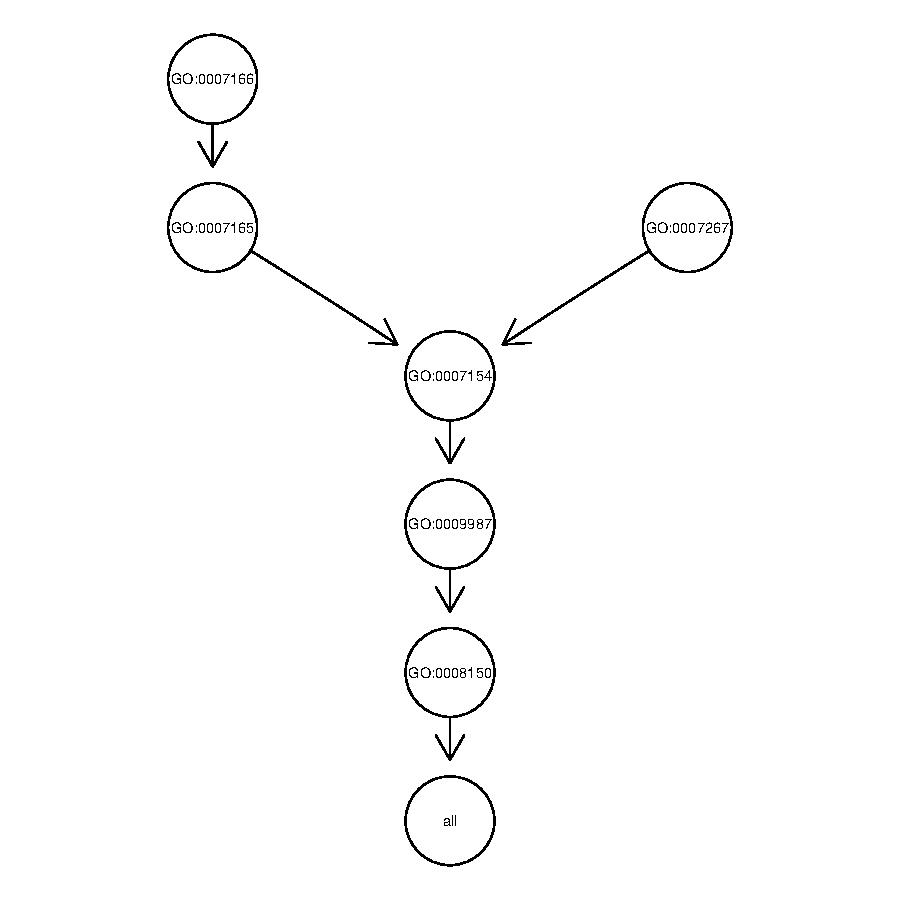
\includegraphics[width=0.6\textwidth]{GOExample.pdf}
\caption{\label{Fig:GOPlot}Example of a GO graph starting with leaves GO:0007166 and GO:0007267.}
\end{center}
\end{figure}

In contrast to the above defined similarity measures Couto et al. \cite{Couto2005GraSM} introduced a concept, which is not based on the minimum subsumer, but on the set of all disjunctive common ancestors. Roughly speaking, the idea is not to consider the common ancestor having the highest information content only, but also others, if they are somehow "separate" from each other, i.e. there is a path to $t$ and $t'$ not passing any other of the disjunctive common ancestors.
\begin{Schunk}
\begin{Sinput}
> getDisjCommAnc("GO:0007166", "GO:0007267")
\end{Sinput}
\begin{Soutput}
[1] "GO:0007154"
\end{Soutput}
\end{Schunk}
In this case the set of disjunctive common ancestors only consists of the minimum subsumer, because any path from the other ancestors to GO:0007166 and GO:0007267 would have to pass the minimum subsumer (see Fig. \ref{Fig:GOPlot}).

Based on the notion of disjunctive common ancestors Resnik's similarity concept can be extended by defining:
\begin{equation}
sim(t,t') = IC_{share}(t,t') = \frac{1}{|DisjCommAnc|}\sum_{t\in DisjCommAnc} IC(t)
\end{equation}
Likewise, Jiang-Conraths's and Lin's measures can be extended as well by replacing $IC_{ms}(t,t')$ by $IC_{share}(t,t')$.
\begin{Schunk}
\begin{Sinput}
> getTermSim(c("GO:0007166", "GO:0007267", "GO:0007584", "GO:0007165", 
+     "GO:0007186"), method = "CoutoResnik", verbose = FALSE)
\end{Sinput}
\begin{Soutput}
           GO:0007166 GO:0007267 GO:0007584 GO:0007165 GO:0007186
GO:0007166  1.0000000  0.3007260  0.2307924  0.3007260  0.3097532
GO:0007267  0.3007260  1.0000000  0.2307924  0.3007260  0.3007260
GO:0007584  0.2307924  0.2307924  1.0000000  0.2307924  0.2307924
GO:0007165  0.3007260  0.3007260  0.2307924  1.0000000  0.3007260
GO:0007186  0.3097532  0.3007260  0.2307924  0.3007260  1.0000000
\end{Soutput}
\end{Schunk}

Finally, it should be mentioned that also the depth and density enriched term similarity by Couto et al. \cite{Couto2003FuSSiMeg} has been integrated into \emph{GOSim}:
\begin{Schunk}
\begin{Sinput}
> setEnrichmentFactors(alpha = 0.5, beta = 0.3)
> getTermSim(c("GO:0007166", "GO:0007267", "GO:0007584", "GO:0007165", 
+     "GO:0007186"), method = "CoutoEnriched", verbose = FALSE)
\end{Sinput}
\begin{Soutput}
           GO:0007166 GO:0007267 GO:0007584 GO:0007165 GO:0007186
GO:0007166  1.0000000  0.1432361  0.1760624  0.1080692  0.1361099
GO:0007267  0.1432361  1.0000000  0.2061625  0.1276006  0.1504305
GO:0007584  0.1760624  0.2061625  1.0000000  0.1577771  0.1843771
GO:0007165  0.1080692  0.1276006  0.1577771  1.0000000  0.1136813
GO:0007186  0.1361099  0.1504305  0.1843771  0.1136813  1.0000000
\end{Soutput}
\end{Schunk}

\subsection{Functional Gene Similarities}

The special strength of \emph{GOSim} lies in the possibility not only to calculate similarities for individual GO terms, but also for genes based on their complete GO anntation. Since \emph{GOSim} version 1.1 for this purpose four basic ideas have been implemented: 
\begin{enumerate}
\item Maximum and average pairwise GO term similarity
\item Average of best matching GO term similarities \cite{Schlicker2006GOFuncSim}.
\item Computation of a so-called \emph{optimal assignment} of terms from one gene to those of another one \cite{FroeSpeerGOKer06}.
\item Embedding of each gene into a feature space defined by the gene's similarity to certain prototype genes  \cite{FroeGO05,FroeSpeerGOKer06}. Within this feature space similarities naturally arise as dot products between the feature vectors. These dot products can be understood as so-called \emph{kernel functions} \cite{SchSmo02}, as used in e.g. Support Vector Machines \cite{CorVap95}.
\end{enumerate}

\subsection{Maximum and Average Pairwise GO Term Similarity}

The idea of the maximum pairwise GO term similarity is straight forward. Given two genes $g$ and $g'$ annotated with GO terms $t_{1},...,t_{n}$ and $t'_{1},...,t'_{m}$ we define the functional similarity between between $g$ and $g'$ as
\begin{eqnarray}
sim_{gene}(g,g') & = & \max_{\begin{array}{c}
i=1,,...,n\\
j=1,...,m\end{array}}sim(t_{i},t'_{j})
\end{eqnarray}
where $sim$ is some similarity measure to compare GO terms $t_i$ and $t'_j$.
Instead of computing the maximum pairwise GO term similarity one may also take the average here.

To normalize the similarities later on, we can peform the transformation
\begin{equation}
sim_{gene}(g,g')\leftarrow\frac{sim_{gene}(g,g')}{\sqrt{sim_{gene}(g,g)sim_{gene}(g',g')}}\label{eq:normalize}
\end{equation}
The consequence will be a similarity of 1 for $g$ with itself and between 0 and 1 for $g$ with any other gene. 
Another possibility is to use the Lin's normalization (see Eq. \ref{eq:Lin})
\begin{equation}
sim_{gene}(g,g')\leftarrow\frac{2sim_{gene}(g,g')}{sim_{gene}(g,g)+sim_{gene}(g',g')}\label{eq:normalize2}
\end{equation}

\subsection{Average of Best Matching GO Term Similarities }

The idea of this approach \cite{Schlicker2006GOFuncSim} is to assign each GO term $t_i$ occuring in gene $g$ to its best matching partner $t'_{\pi{i}}$ in gene $g'$. Hence multiple GO terms from gene $g$ can be assigned to one GO term from gene $g'$. A similarity score is computed by taking the average similarity of assigned GO terms. Since, however, genes can have an unequal number of GO terms the result depends on whether GO terms of gene $g$ are assigned to those of gene $g'$ or vice versa. Hence, in \cite{Schlicker2006GOFuncSim} it was proposed to either take the maximum or the average of both similarity scores. Both strategies are implemented in \emph{GOSim}. 

\subsubsection{Optimal Assignment Gene Similarities}

To elucidate the idea of the optimal assignment, consider the GO terms associated with gene "8614" on one hand and gene "2852" on the other hand:
\begin{Schunk}
\begin{Sinput}
> getGOInfo(c("8614", "2852"))
\end{Sinput}
\begin{Soutput}
$`8614`
$`8614`$`GO:0007166`
GOID: GO:0007166
Term: cell surface receptor linked signal transduction
Ontology: BP
Definition: Any series of molecular signals initiated by the binding of
    an extracellular ligand to a receptor on the surface of the target
    cell.

$`8614`$`GO:0007267`
GOID: GO:0007267
Term: cell-cell signaling
Ontology: BP
Definition: Any process that mediates the transfer of information from
    one cell to another.
Synonym: cell-cell signalling

$`8614`$`GO:0007584`
GOID: GO:0007584
Term: response to nutrient
Ontology: BP
Definition: A change in state or activity of a cell or an organism (in
    terms of movement, secretion, enzyme production, gene expression,
    etc.) as a result of a nutrient stimulus.
Synonym: response to nutrients
Synonym: nutritional response pathway


$`2852`
$`2852`$`GO:0007165`
GOID: GO:0007165
Term: signal transduction
Ontology: BP
Definition: The cascade of processes by which a signal interacts with a
    receptor, causing a change in the level or activity of a second
    messenger or other downstream target, and ultimately effecting a
    change in the functioning of the cell.
Synonym: signaling
Synonym: signalling

$`2852`$`GO:0007186`
GOID: GO:0007186
Term: G-protein coupled receptor protein signaling pathway
Ontology: BP
Definition: The series of molecular signals generated as a consequence
    of a G-protein coupled receptor binding to its physiological
    ligand.
Synonym: G protein coupled receptor protein signaling pathway
Synonym: G protein coupled receptor protein signalling pathway
Synonym: G-protein coupled receptor protein signalling pathway
Synonym: G-protein-coupled receptor protein signaling pathway
Synonym: G-protein-coupled receptor protein signalling pathway
Synonym: GPCR protein signaling pathway
Synonym: GPCR protein signalling pathway
\end{Soutput}
\end{Schunk}
Given a similarity concept $sim$ to compare individual GO terms, the idea is now to assign each term of the gene having fewer annotation to exactly one term of the other gene such that the overall similarity is maximized. Hence, in the optimal assignment 
More formally optimal assignment problem can be stated as follows: Let $\pi$ be some permutation of either an $n$-subset of natural numbers
$\{1,...,m\}$ or an $m$-subset of natural numbers $\{1,...,n\}$ (this will
be clear from context). Then we are looking for the quantity
\begin{equation}
sim_{gene}(g,g')=\left\{ \begin{array}{cc}
\max_{\pi}\sum_{i=1}^{n}sim(t_{i},t'_{\pi(i)}) & \textrm{if }m>n\\
\max_{\pi}\sum_{j=1}^{m}sim(t_{\pi(j)},t'_{j}) & \textrm{ otherwise}
\end{array}\right.\label{eq:OAKernel}
\end{equation}
The computation of (\ref{eq:OAKernel}) corresponds to the solution
of the classical maximum weighted bipartite matching (optimal assignment)
problem in graph theory and can be carried out in $O(\max(n,m)^{3})$
time \cite{LEDABook99}. 
To prevent that larger lists of terms automatically
achieve a higher similarity we may further $sim_{gene}$ divide \ref{eq:OAKernel} by $\max(m,n)$.

In our example, using Lin's GO term similarity measure the following assignments are found:
\begin{eqnarray}
\mathtt{GO:0007165} & \to & \mathtt{GO:0007267}\\
\mathtt{GO:0007186} & \to & \mathtt{GO:0007166}
\end{eqnarray}
The resulting similarity matrix is:
\begin{Schunk}
\begin{Sinput}
> getGeneSim(c("8614", "2852"), similarity = "OA", similarityTerm = "Lin", 
+     verbose = FALSE)
\end{Sinput}
\begin{Soutput}
          8614      2852
8614 1.0000000 0.5839585
2852 0.5839585 1.0000000
\end{Soutput}
\end{Schunk}

Note the difference to a gene similarity that is just based on the maximum GO term similarity and to a gene similarity that is based on the average of best matching GO terms:
\begin{Schunk}
\begin{Sinput}
> getGeneSim(c("8614", "2852"), similarity = "max", similarityTerm = "Lin", 
+     verbose = FALSE)
\end{Sinput}
\begin{Soutput}
         8614     2852
8614 1.000000 0.967612
2852 0.967612 1.000000
\end{Soutput}
\begin{Sinput}
> getGeneSim(c("8614", "2852"), similarity = "funSimMax", similarityTerm = "Lin", 
+     verbose = FALSE)
\end{Sinput}
\begin{Soutput}
          8614      2852
8614 1.0000000 0.9465487
2852 0.9465487 1.0000000
\end{Soutput}
\end{Schunk}

\subsubsection{Feature Space Embedding of Gene Products}

To calculate the feature vectors for each gene we can either define certain prototype genes a priori or we use one of the heuristics implemented in the function {\tt selectPrototypes}. The default behavior is to select the 250 best annotated genes, i.e. which have been annotated with GO terms most often:
\begin{Schunk}
\begin{Sinput}
> proto = selectPrototypes(verbose = FALSE)
\end{Sinput}
\end{Schunk}

We now calculate for each gene $g$ feature vectors $\phi(g)$  by using their similarity to all prototypes $p_1,...,p_n$:
\begin{equation}
\phi(g) = (sim'(g,p_1),...,sim'(g,p_n))^T
\end{equation}
Here $sim'$ by default is the maximum pairwise GO term similarity. Alternatively, one can use the optimal assignment similarity for $sim'$ as well. Both similarity measures can by itself again be combined with arbitrary GO term similarity concepts. The default is the Jiang-Conrath term similarity.

Because the feature vectors are very high-dimensional we usually perform a principal component analysis (PCA) to project the data into a lower dimensional subspace:
\begin{Schunk}
\begin{Sinput}
> PHI = getGeneFeaturesPrototypes(genes, prototypes = proto, verbose = FALSE)
\end{Sinput}
\end{Schunk}

This uses the above define prototypes to calculate feature vectors and performs a PCA afterwards. The number of principal components is chosen such that at least 95\% of the total variance in feature space can be explained (this is a relatively conservatve criterion). 

We can now plot our genes in the space spanned by the first 2 principal components to get an impression of the relative  "position" of the genes to each other in the feature space (see Fig. \ref{Fig:PCAPlot}). The feature vectors are normalized to Euclidian norm 1 by default:
\begin{Schunk}
\begin{Sinput}
> x = seq(min(PHI$features[, 1]), max(PHI$features[, 1]), length.out = 100)
> y = seq(min(PHI$features[, 2]), max(PHI$features[, 2]), length.out = 100)
> plot(x, y, xlab = "principal component 1", ylab = "principal component 2", 
+     type = "n")
> text(PHI$features[, 1], PHI$features[, 2], labels = genes)
\end{Sinput}
\end{Schunk}

\begin{figure}
\begin{center}
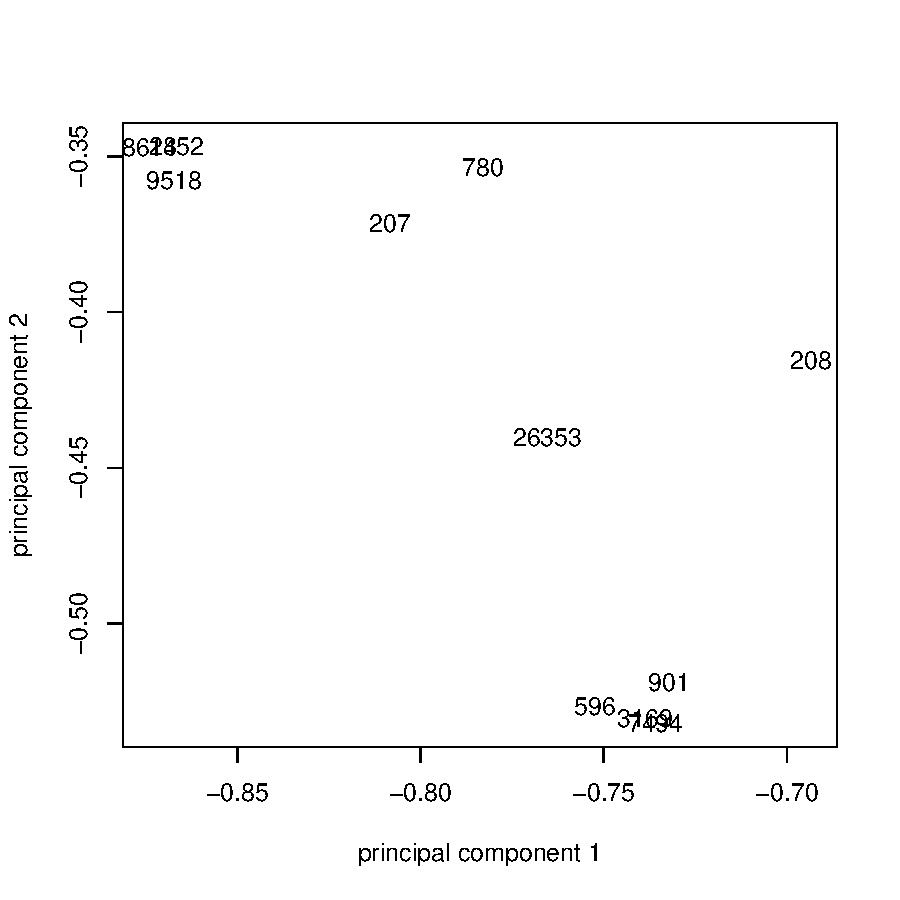
\includegraphics[width=0.5\textwidth]{GOPCAExample.pdf}
\caption{\label{Fig:PCAPlot}Embedding of the genes into the feature space spanned by the first 2 principal components}
\end{center}
\end{figure}

Finally, we can directly calculate the similarities of the genes to each other, this time using the Resnik's GO term similarity concept. These similarities may then be used to cluster genes with respect to their function:
\begin{Schunk}
\begin{Sinput}
> sim = getGeneSimPrototypes(genes, prototypes = proto, similarityTerm = "Resnik", 
+     verbose = FALSE)
> h = hclust(as.dist(1 - sim$similarity), "ward")
> plot(h, xlab = "")
\end{Sinput}
\end{Schunk}

This produces a hierarchical clustering of all genes using Ward's method (see Fig. \ref{Fig:GOCluster}).

\begin{figure}
\begin{center}
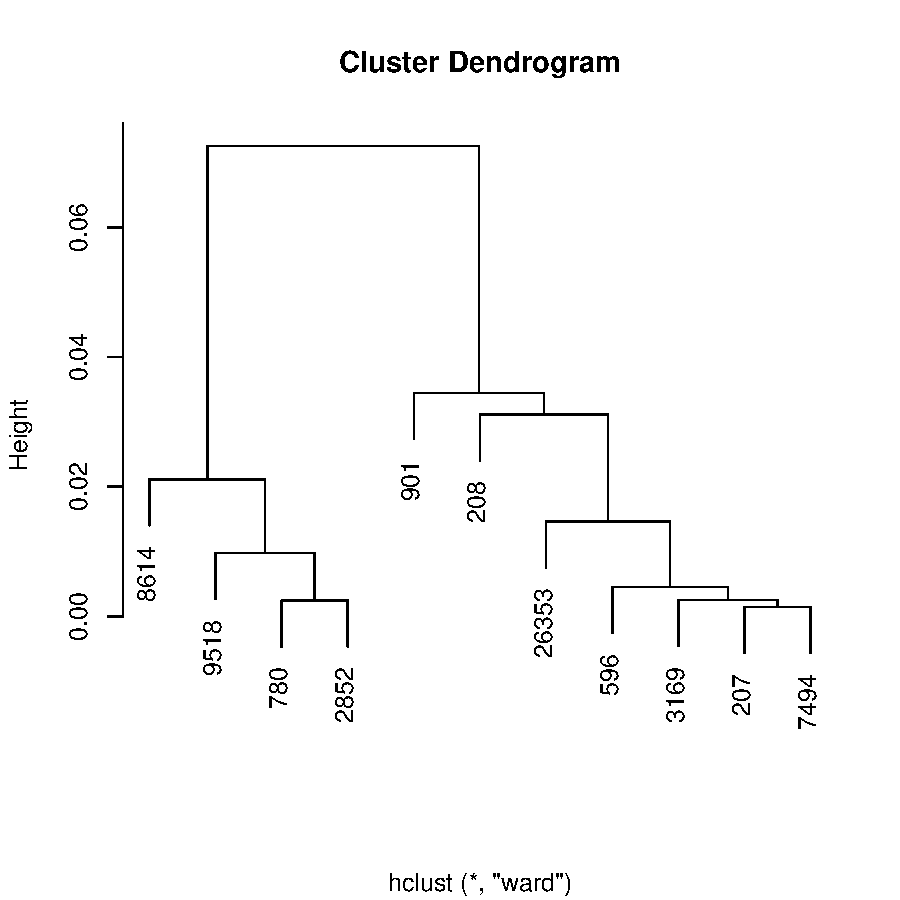
\includegraphics[width=0.5\textwidth]{GOClusterExample.pdf}
\caption{\label{Fig:GOCluster}Possible functional clustering of the genes using Ward's method.}
\end{center}
\end{figure}

It should be mentioned that up to now all similarity computations were performed within the ontology "biological process". One could imagine to combine functional similarities between gene products with regard to different taxonomies. An obvious way for doing so would be to consider the sum of the respective similarities:
\begin{equation}
sim_{total}(g,g') = sim_{Ontology1}(g,g') + sim_{Ontology2}(g,g')
\end{equation}
Of course, one could also use a weighted averaging scheme here, if desired.


\subsection{Cluster Evaluations}

\emph{GOSim} has the possibility to evaluate a given clustering of genes or terms by means of their GO similarities. Supposed, based on other experiments (e.g. microarry), we have decided to put genes "8614", "9518", "780", "2852" in one group, genes "3169", "207", "7494", "596" in a second and the rest in a third group. Then we can ask ourselves, how similar these groups are with respect to their GO annotations:
\begin{Schunk}
\begin{Sinput}
> ev = evaluateClustering(c(2, 3, 2, 3, 1, 2, 1, 1, 3, 1, 2), sim$similarity)
> plot(ev$clustersil, main = "")
\end{Sinput}
\end{Schunk}
\begin{figure}[t]
\begin{center}
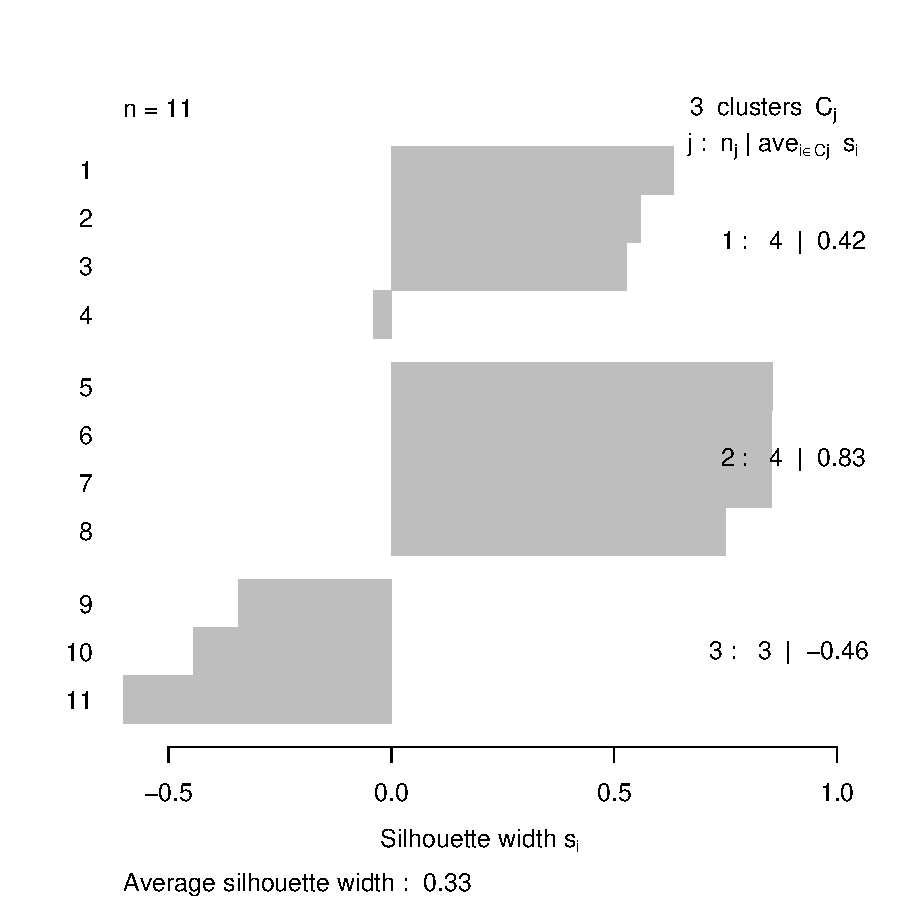
\includegraphics[width=0.5\textwidth]{GOClustersil.pdf}
\caption{\label{Fig:GOClustersil}Silhouette plot of a possible given grouping of genes.}
\end{center}
\end{figure}

A good indiciation of the clustering qualitiy can be obtained by looking at the cluster silhouettes \cite{rousseeuw87} (see Fig. \ref{Fig:GOClustersil}). This shows that clusters 1 and 2 are relatively homogenous with respect to the functional similarity of the genes contained in it, while the genes in cluster 3 are more dissimilar.

\subsection{GO Enrichment Analysis}

Since version 1.1 \emph{GOSim} also offers the possibility of a GO enrichemnt analysis. Suppose, we may now want to get a clearer picture of the genes involved in cluster 1. For this purpose we use the topGO tool \cite{Alexa2006topGO}.
\begin{Schunk}
\begin{Sinput}
> gomap <- get("gomap", env = GOSimEnv)
> allgenes = unique(c(sample(names(gomap), 1000), genes))
> analyzeCluster(c("8614", "9518", "780", "2852"), allgenes)
\end{Sinput}
\begin{Soutput}
Package SparseM (0.73) loaded.  To cite, see citation("SparseM")

groupGOTerms: 	GOBPTerm, GOMFTerm, GOCCTerm environments built.

Building most specific GOs .....	( 822 GO terms found. )

Build GO DAG topology ..........	( 1853 GO terms and 3063 relations. )

Annotating nodes ...............	( 851 genes annotated to the GO terms. )

			 -- Elim Algorithm -- 

		 the algorithm is scoring 34 nontrivial nodes
		 parameters: 
			 test statistic:  Fisher test 
			 cutOff:  0.01 

	 Level 8:	2 nodes to be scored	(0 eliminated genes)

	 Level 7:	3 nodes to be scored	(2 eliminated genes)

	 Level 6:	5 nodes to be scored	(2 eliminated genes)

	 Level 5:	5 nodes to be scored	(3 eliminated genes)

	 Level 4:	7 nodes to be scored	(89 eliminated genes)

	 Level 3:	7 nodes to be scored	(103 eliminated genes)

	 Level 2:	4 nodes to be scored	(103 eliminated genes)

	 Level 1:	1 nodes to be scored	(103 eliminated genes)
$GOTerms
$GOTerms$`GO:0007179`
GOID: GO:0007179
Term: transforming growth factor beta receptor signaling pathway
Ontology: BP
Definition: The series of molecular signals generated as a consequence
    of a transforming growth factor beta receptor binding to one of its
    physiological ligands.
Synonym: TGF-beta receptor signaling pathway
Synonym: TGF-beta receptor signalling pathway
Synonym: TGFbeta receptor signaling pathway
Synonym: TGFbeta receptor signalling pathway
Synonym: transforming growth factor beta receptor signalling pathway

$GOTerms$`GO:0007267`
GOID: GO:0007267
Term: cell-cell signaling
Ontology: BP
Definition: Any process that mediates the transfer of information from
    one cell to another.
Synonym: cell-cell signalling

$GOTerms$`GO:0007584`
GOID: GO:0007584
Term: response to nutrient
Ontology: BP
Definition: A change in state or activity of a cell or an organism (in
    terms of movement, secretion, enzyme production, gene expression,
    etc.) as a result of a nutrient stimulus.
Synonym: response to nutrients
Synonym: nutritional response pathway

$GOTerms$`GO:0007166`
GOID: GO:0007166
Term: cell surface receptor linked signal transduction
Ontology: BP
Definition: Any series of molecular signals initiated by the binding of
    an extracellular ligand to a receptor on the surface of the target
    cell.


$p.values
 GO:0007179  GO:0007267  GO:0007584  GO:0007166 
0.009384116 0.003712815 0.004700353 0.001042917 
\end{Soutput}
\end{Schunk}
The result shows that the four genes are mainly involved in cell-cell signaling, in an enzyme linked receptor protein signaling pathway and in the response to nutrient.

\bibliographystyle{plain}
\bibliography{/mountpoints/stoneage/home/froehlih/Papers/references,/mountpoints/stoneage/home/froehlih/Papers/GOCluster}

\end{document}
